\documentclass[12pt]{article}

%-------------PACKAGES------------- 
\usepackage[margin=1in]{geometry} 
\usepackage{amsmath,amsthm,amssymb}
\usepackage{pgfplots}
\usepackage{float}
\usepackage{braket}
\usepackage{titling}
\usepackage{tikz}
\usepackage{mathtools}
\usepackage{listings}
\usepackage{color}
\usepackage{caption}
\usepackage{subcaption}
\usepackage{algorithm,algpseudocode}
\usetikzlibrary{shapes,arrows,chains}
\usetikzlibrary[calc]

%-------------FORMATTING-------------
\setlength{\droptitle}{-5em} 
\setlength{\parindent}{0pt}
\def\LW{\dimexpr.25\linewidth-.5em} 
\tikzstyle{line} = [draw, -latex']
 
%--------------COMMANDS--------------
\newcommand{\N}{\mathbb{N}}
\newcommand{\Z}{\mathbb{Z}}
\newcommand{\R}{\mathbb{R}}
\newcommand{\C}{\mathbb{C}}
%\renewcommand{\qedsymbol}{\filledbox}

\DeclarePairedDelimiter \abs{\lvert}{\rvert}%
\DeclarePairedDelimiter \norm{\lVert}{\rVert}%

%------------ENVIRONMENTS------------- 
\newenvironment{theorem}[2][]{\begin{trivlist}
\item[{\bfseries #1}\hskip \labelsep {\bfseries #2.}]}{\end{trivlist}}
\newenvironment{lemma}[2][Lemma]{\begin{trivlist}
\item[\hskip \labelsep {\bfseries #1}\hskip \labelsep {\bfseries #2.}]}{\end{trivlist}}
\newenvironment{exercise}[2][Exercise]{\begin{trivlist}
\item[\hskip \labelsep {\bfseries #1}\hskip \labelsep {\bfseries #2.}]}{\end{trivlist}}
\newenvironment{reflection}[2][Reflection]{\begin{trivlist}
\item[\hskip \labelsep {\bfseries #1}\hskip \labelsep {\bfseries #2.}]}{\end{trivlist}}
\newenvironment{proposition}[2][Proposition]{\begin{trivlist}
\item[\hskip \labelsep {\bfseries #1}\hskip \labelsep {\bfseries #2.}]}{\end{trivlist}}
\newenvironment{corollary}[2][Corollary]{\begin{trivlist}
\item[\hskip \labelsep {\bfseries #1}\hskip \labelsep {\bfseries #2.}]}{\end{trivlist}}
\theoremstyle{remark}
\newtheorem*{remark}{Remark}

%-------------CODE-STYLE------------
\definecolor{dkgreen}{rgb}{0,0.6,0}
\definecolor{gray}{rgb}{0.5,0.5,0.5}
\definecolor{mauve}{rgb}{0.58,0,0.82}
\lstset{frame=tb,
	language=C++,
	aboveskip=3mm,
	belowskip=3mm,
	showstringspaces=false,
	columns=flexible,
	basicstyle={\small\ttfamily},
	numbers=none,
	numberstyle=\tiny\color{gray},
	keywordstyle=\color{blue},
	commentstyle=\color{dkgreen},
	stringstyle=\color{mauve},
	breaklines=true,
	breakatwhitespace=true,
	tabsize=3
}

\lstset{
	morekeywords={end}
}

%------------------------------------ 
%---------START-OF-DOCUMENT----------
%------------------------------------
\begin{document}
 
\title{Program 4}
\author{David Miller \\ 
MAD5403: Foundations of Computational Math I} 
 
\maketitle

\section{Executive Summary}

In this program we investigate extrapolation between Simpson's first and Simpson's second and Simpson's first and Open Netwon Cotes that uses 3 points. We alos investigate the accuracy and convergence between Romberg's method and Trapezoidal with refinement. An analysis is given for these and results are presented at the end to give numerical evidence of our analysis. 

\section{Statement of Problem}

This program has two main parts
\begin{enumerate}
	\item Compute error forms for two extrapolation methods: $I_{new} = \frac{9}{5}I_{ss} - \frac{4}{5}I_{sf}$ and $I_{new} = \frac{7}{15}I{sf} + \frac{8}{15}I_{o2}$ determine if they are Newton Cotes methods and/or if they are interpolatory quadrature
	\item Numerically test and investigate Trapezoidal method with refinement vs Romberg's method and determine the relation between the two
\end{enumerate}
The former is analysis that is done out in the section 3 and the latter is presented in sections 4, 5, and 6.  Numerical tests were all carried out in double precision.	

\newpage 

\section{Description of Mathematics}


In this assignment we use four quadrature methods : Simpson's first, Simpson's second, and Open Newton Cotes formula that uses 3 points, and Trapezoidal. We use  the notation $f_i^{(m)}$ where $f(x_i)$ is the function evaluation for the mesh point $x_i$ in method $m$. 
\begin{align*}
& \textbf{Simpson's First Rule} \hskip 12.5cm \\ \\
& I_{sf} = \frac{1}{3}h_{sf}\bigg[f_0^{(sf) 4f_1^{(sf)}} + f_2^{(sf)}\bigg] = (b-a)\bigg[\frac{1}{6}f_0^{(sf)} + \frac{2}{3}f_1^{(sf)} + f_2^{(sf)}\bigg], \quad E_{sf} = -\frac{1}{2880}(b-a)^5f^{(4)}(\eta) \\ \\
& \text{where $h_{sf} = (b-a)/2$.} \\ \\
& \textbf{Simpson's Second Rule} \\ \\
& I_{ss} = \frac{3}{8}h_{ss}\bigg[f_0^{(ss)} + 3f_1^{(ss)} + 3f_2^{(ss)} + f_3^{(ss)}\bigg] = (b-a)\bigg[\frac{1}{8}f_0^{(ss)} + \frac{3}{8}f_0^{(ss)} + \frac{3}{8}f_2^{(ss)} + \frac{1}{8}f_0^{(ss)}\bigg], \\ \\
& E_{ss} = -\frac{1}{6480}(b-a)^5f^{(4)}(\xi) \\ \\
& \text{where $h_{ss} = (b-a)/3$} \\ \\
& \textbf{Open Newton Cotes that uses 3 points} \\ \\
& I_{o2} = \frac{4}{3}h_{o2}\bigg[2f_0^{(o2)} - f_1^{(o2)} + 2f_2^{(o2)}\bigg] = (b-a)\bigg[\frac{2}{3}f_0^{(o2)} - \frac{1}{3}f_1^{(o2)} + \frac{2}{3}f_2^{(o2)}\bigg], \quad E_{o2} = \frac{7}{23040}(b-a)^5f^{(4)}(\mu) \\ \\
& \text{where $h_{o2} = (b-a)/4$} \\ \\
& \textbf{Trapezoidal Rule} \hskip 13cm \\ \\
& I_{t} = \frac{1}{2}h_{t}\bigg[f_0^{t} + f_1^{(t)}\bigg] = (b-a)\bigg[\frac{1}{2}f_0^{(t)} + \frac{1}{2}f_1^{(t)}\bigg], \quad E_t = -\frac{1}{12}f^{(2)}(\chi) \\ \\
& \text{where $h_t = b-a$}
\end{align*}
We will also make use of the following theorem
\begin{theorem}{Theorem 1}
	A quadrature formula using $n + 1$ distinct points is an
	interpolatory quadrature formula if and only if it has degree of exactness greater than or equal to $n$
\end{theorem}
\newpage

\subsection{Simpson's First and Simpson's Second}

Simpson's first and Simpson's second methods can be combined
\begin{align}
	I_{new} = \frac{9}{5}I_{ss} - \frac{4}{5}I_{sf}
\end{align} 
where its error can be expressed as $I - I_{new} = Ch^df^{(s)} + \mathcal{O}(h^{d+1})$. To figure out the constant $C$, power $d$, and order of derivative $s$ we first need to determine an expression for $I_{new}$. Letting $h = \frac{b-a}{2}$ we have
\begin{center}
	\begin{tikzpicture}	
	\draw (0,0) -- (4,0) -- (4,1) -- (0,1) -- (0,0);
	\draw (4,0) -- (8,0) -- (8,1) -- (4,1) -- (4,0);
	\draw (6,1) -- (6,0);
	\draw (8,0) -- (12,0) -- (12,1) -- (8,1) -- (8,0);
	
	\draw[latex'-latex', very thick] (0.1,-0.25) to (3.9,-0.25);
	\node[text width=2cm] at (2.75,-0.6) {$\frac{2h}{3}$};
	\draw[latex'-latex', very thick] (4.1,-0.25) to (5.9,-0.25);
	\node[text width=2cm] at (5.75,-0.6) {$\frac{h}{3}$};
	\draw[latex'-latex', very thick] (6.1,-0.25) to (7.9,-0.25);
	\node[text width=2cm] at (7.75,-0.6) {$\frac{h}{3}$};
	\draw[latex'-latex', very thick] (8.1,-0.25) to (11.9,-0.25);
	\node[text width=2cm] at (10.75,-0.6) {$\frac{2h}{3}$};
	
	\node[text width=2cm] at (.8,1.35) {$x_0$};
	\node[text width=2cm] at (4.8,1.35) {$x_1$};
	\node[text width=2cm] at (6.8,1.35) {$x_2$};
	\node[text width=2cm] at (8.8,1.35) {$x_3$};
	\node[text width=2cm] at (12.8,1.35) {$x_4$};
	\end{tikzpicture}
\end{center}
where $x_0, x_2,$ and $x_4$ come from $I_{sf}$ and $x_0, x_1, x_3,$ and $x_4$ come from $I_{ss}$.  We have that $I_{new}$ is
\begin{align*}
	I_{new} & = \frac{9}{5}I_{ss} - \frac{4}{5}I_{sf} \\
	& = \frac{9}{5}\bigg[\frac{b-a}{8}\bigg(f_0 + 3f_1 + 3f_3 + f_4\bigg)\bigg] - \frac{4}{5}\bigg[\frac{b-a}{6}\bigg(f_0 + 4f_2 + f_4\bigg)\bigg] \\
	& = \frac{9(b-a)}{40}\bigg(f_0 + 3f_1 + 3f_3 + f_4\bigg) - \frac{4}{30}\bigg(f_0 + 4f_2 + f_4\bigg) \\
	& = \frac{b-a}{120}\bigg(11f_0 + 81f_1 - 64f_2 + 81f_3 + 11f_4 \bigg) \\
	& = \frac{h}{60}\bigg(11f_0 + 81f_1 - 64f_2 + 81f_3 + 11f_4 \bigg)
\end{align*}
All that is left is to find an expression for $I$. We can do this by finding an expression for $f(x)$ by Taylor expanding around $x_2$ and integrating it.
\begin{align*}
	f(x) & = f_2 + f^{(1)}_2\frac{(x-x_2)}{1!} + f^{(2)}_2\frac{(x-x_2)^2}{2!} + f^{(3)}_2\frac{(x-x_2)^3}{3!} + f^{(4)}_2\frac{(x-x_2)^4}{4!}
	\\ & + f^{(5)}_2\frac{(x-x_2)^5}{5!} + f^{(6)}_2\frac{(x-x_2)^6}{6!} + \mathcal{O}((x-x_2)^7) \\
	& = f_2 + f^{(1)}_2h + f_2^{(2)}\frac{h^2}{2!} + f_2^{(3)}\frac{h^3}{3!} + f_2^{(4)}\frac{h^4}{4!} + f_2^{(5)}\frac{h^5}{5!} + f_2^{(6)}\frac{h^6}{6!} + \mathcal{O}(h^7)
\end{align*}
To integrate we first do a change of variables by letting $x = x_2 + sh$ for $-1 \leq s \leq 1$. Therefore we have $dx = hds$ and end up with
\begin{align*}
	I & = h\int\limits_{-1}^1 f(s) \, ds
	\\ & = h\int\limits_{-1}^1 f_2 + f^{(1)}_2\frac{sh}{1!} + f_2^{(2)}\frac{(sh)^2}{2!} + f_2^{(3)}\frac{(sh)^3}{3!} + f_2^{(4)}\frac{(sh)^4}{4!} + f_2^{(5)}\frac{(sh)^5}{5!} + f_2^{(6)}\frac{(sh)^6}{6!} \, ds
	\\ & = h\bigg(2f_2 + f_2^{(2)}\frac{2h^2}{3!} + f_2^{(4)}\frac{2h^4}{5!} + f_2^{(6)}\frac{2h^6}{7!}\bigg)
\end{align*}
Combining the expression for $I$ and $I_{new}$ we get
\begin{align*}
	I - I_{new} & = h\bigg(2f_2 + f_2^{(2)}\frac{2h^2}{3!} + f_2^{(4)}\frac{2h^4}{5!} + f_2^{(6)}\frac{2h^6}{7!}\bigg) 
	\\ & - \frac{h}{60}\bigg(11f_0 + 81f_1 - 64f_2 + 81f_3 + 11f_4 \bigg)
	\\ & = h\bigg(2f_2 + f_2^{(2)}\frac{2h^2}{3!} + f_2^{(4)}\frac{2h^4}{5!} + f_2^{(6)}\frac{2h^6}{7!}\bigg)
	\\ & - \frac{h}{60}\bigg[11\bigg(f_2 - f_2^{(1)}\frac{h}{1!} + f_2^{(2)}\frac{h^2}{2!} - f_2^{(3)}\frac{h^3}{3!} + f_2^{(4)}\frac{h^4}{4!} - f_2^{(5)}\frac{h^5}{5!} + f_2^{(6)}\frac{h^6}{6!}\bigg)
	\\ & + 81\bigg(f_2 - f_2^{(1)}\frac{h}{1!3} + f_2^{(2)}\frac{h^2}{2!3^2} - f_2^{(3)}\frac{h^3}{3!3^3} + f_2^{(4)}\frac{h^4}{4!3^4} - f_2^{(5)}\frac{h^5}{5!3^5} + f_2^{(6)}\frac{h^6}{6!3^6}\bigg)
	\\ & - 64f_2
	\\ & + 81\bigg(f_2 + f_2^{(1)}\frac{h}{1!3} + f_2^{(2)}\frac{h^2}{2!3^2} + f_2^{(3)}\frac{h^3}{3!3^3} + f_2^{(4)}\frac{h^4}{4!3^4} + f_2^{(5)}\frac{h^5}{5!3^5} + f_2^{(6)}\frac{h^6}{6!3^6}\bigg)
	\\ & + 11\bigg(f_2 + f_2^{(1)}\frac{h}{1!} + f_2^{(2)}\frac{h^2}{2!} + f_2^{(3)}\frac{h^3}{3!} + f_2^{(4)}\frac{h^4}{4!} + f_2^{(5)}\frac{h^5}{5!} + f_2^{(6)}\frac{h^6}{6!}\bigg)\bigg]
\end{align*}
Gathering like terms and simplifying we end up with the expression
\begin{align}
	I - I_{new} = -\frac{1}{8505}h^7f^{(6)}_2 + \mathcal{O}(h^8)
\end{align}
which implies
\begin{align*}
C = -\frac{1}{8505}, \quad d = 7, \quad s = 6
\end{align*}
Since the degree fo exactness is 5, by Theorem 1 $I_{new} = \frac{9}{5}I_{ss} - \frac{4}{5}I_{sf}$ is a polynomial interpolation quadrature method. However, $I_{new}$ is not Newton Cotes method since it interpolates at non-uniform mesh points. 

\newpage

\subsection{Simpson's First and Open-2}

Simpson's first and Open-2 methods can be combined
\begin{align}
I_{new} = \alpha_{sf}I_{sf} - \alpha_{O2}I_{O2}
\end{align} 
where $\alpha_1$ and $\alpha_2$ are obtained via
\begin{align*}
	\alpha_{sf} = \frac{C_{O2}}{C_{O2} - C_{sf}} = \frac{-\frac{7}{23040}}{-\frac{7}{23040} - \frac{1}{2880}} = \frac{7}{15}, \quad \alpha_{O2} = \frac{C_{sf}}{C_{sf} - C_{O2}} = \frac{\frac{1}{2880}}{\frac{1}{2880}+\frac{7}{23040}} = \frac{8}{15}
\end{align*}
The error can be expressed as $I - I_{new} = Ch^df^{(s)} + \mathcal{O}(h^{d+1})$. To figure out the constant $C$, power $d$, and order of derivative $s$ we first need to determine an expression for $I_{new}$. Letting $h = \frac{b-a}{2}$ we have
\begin{center}
	\begin{tikzpicture}	
	\draw (0,0) -- (3,0) -- (3,1) -- (0,1) -- (0,0);
	\draw (3,0) -- (6,0) -- (6,1) -- (3,1) -- (3,0);
	\draw (6,0) -- (9,0) -- (9,1) -- (6,1) -- (6,0);
	\draw (9,0) -- (12,0) -- (12,1) -- (9,1) -- (9,0);
	
	\draw[latex'-latex', very thick] (0.1,-0.25) to (2.9,-0.25);
	\node[text width=2cm] at (2.375,-0.6) {$\frac{h}{2}$};
	\draw[latex'-latex', very thick] (3.1,-0.25) to (5.9,-0.25);
	\node[text width=2cm] at (5.25,-0.6) {$\frac{h}{2}$};
	\draw[latex'-latex', very thick] (6.1,-0.25) to (8.9,-0.25);
	\node[text width=2cm] at (8.5,-0.6) {$\frac{h}{2}$};
	\draw[latex'-latex', very thick] (9.1,-0.25) to (11.9,-0.25);
	\node[text width=2cm] at (11.375,-0.6) {$\frac{h}{2}$};
	
	\node[text width=2cm] at (.8,1.35) {$x_0$};
	\node[text width=2cm] at (3.8,1.35) {$x_1$};
	\node[text width=2cm] at (6.8,1.35) {$x_2$};
	\node[text width=2cm] at (9.8,1.35) {$x_3$};
	\node[text width=2cm] at (12.8,1.35) {$x_4$};
	\end{tikzpicture}
\end{center}
where $x_0, x_2,$ and $x_4$ come from $I_{sf}$ and $x_1, x_2, x_3,$ and $x_4$ come from $I_{o2}$. We have that $I_{new}$ is
\begin{align*}
	I_{new} & = \frac{7}{15}I_{sf} + \frac{8}{15}I_{o2} 
	\\ & = \frac{7}{15}\bigg[\frac{b-a}{6}\bigg(f_0 + 4f_2 + f_4\bigg)\bigg] + \frac{8}{15}\bigg[\frac{b-a}{3}\bigg(2f_1 - f_2 + f_3\bigg)\bigg]
	\\ & = \frac{7(b-a)}{90}\bigg(f_0 + 4f_2 + f_4\bigg) + \frac{16(b-a)}{90}\bigg(2f_1 - f_2 + 2f_3\bigg)
	\\ & = \frac{b-a}{90}\bigg(7f_0 + 32f_1 + 12f_2 + 32F_3 + 7f_4\bigg)
	\\ & = \frac{h}{45}\bigg(7f_0 + 32f_1 + 12f_2 + 32F_3 + 7f_4\bigg)
\end{align*}
All that is left is to find an expression for $I$. We can do this by finding an expression for $f(x)$ by Taylor expanding around $x_2$ and integrating it.
\begin{align*}
f(x) & = f_2 + f^{(1)}_2\frac{(x-x_2)}{1!} + f^{(2)}_2\frac{(x-x_2)^2}{2!} + f^{(3)}_2\frac{(x-x_2)^3}{3!} + f^{(4)}_2\frac{(x-x_2)^4}{4!}
\\ & + f^{(5)}_2\frac{(x-x_2)^5}{5!} + f^{(6)}_2\frac{(x-x_2)^6}{6!} + \mathcal{O}((x-x_2)^7) \\
& = f_2 + f^{(1)}_2h + f_2^{(2)}\frac{h^2}{2!} + f_2^{(3)}\frac{h^3}{3!} + f_2^{(4)}\frac{h^4}{4!} + f_2^{(5)}\frac{h^5}{5!} + f_2^{(6)}\frac{h^6}{6!} + \mathcal{O}(h^7)
\end{align*}
To integrate we first do a change of variables by letting $x = x_2 + sh$ for $-1 \leq s \leq 1$. Therefore we have $dx = hds$ and end up with
\begin{align*}
I & = h\int\limits_{-1}^1 f(s) \, ds
\\ & = h\int\limits_{-1}^1 f_2 + f^{(1)}_2\frac{sh}{1!} + f_2^{(2)}\frac{(sh)^2}{2!} + f_2^{(3)}\frac{(sh)^3}{3!} + f_2^{(4)}\frac{(sh)^4}{4!} + f_2^{(5)}\frac{(sh)^5}{5!} + f_2^{(6)}\frac{(sh)^6}{6!} \, ds
\\ & = h\bigg(2f_2 + f_2^{(2)}\frac{2h^2}{3!} + f_2^{(4)}\frac{2h^4}{5!} + f_2^{(6)}\frac{2h^6}{7!}\bigg)
\end{align*}
Combining the expression for $I$ and $I_{new}$ we get
\begin{align*}
	I - I_{new} & = h\bigg(2f_2 + f_2^{(2)}\frac{2h^2}{3!} + f_2^{(4)}\frac{2h^4}{5!} + f_2^{(6)}\frac{2h^6}{7!}\bigg)
	\\ & - \frac{h}{45}\bigg(7f_0 + 32f_1 + 12f_2 + 32F_3 + 7f_4\bigg)
	\\ & = h\bigg(2f_2 + f_2^{(2)}\frac{2h^2}{3!} + f_2^{(4)}\frac{2h^4}{5!} + f_2^{(6)}\frac{2h^6}{7!}\bigg)
	\\ & - \frac{h}{45}\bigg[7\bigg(f_2 - \frac{h}{1!}f_2^{(1)} + \frac{h^2}{2!}f_2^{(2)} - \frac{h^3}{3!}f_2^{(3)} + \frac{h^4}{4!}f_2^{(4)} - \frac{h^5}{5!}f_2^{(5)} + \frac{h^6}{6!}f_2^{(6)} \bigg)
	\\ & + 32\bigg(f_2 - \frac{h}{1!2}f_2^{(1)} + \frac{h^2}{2!2^2}f_2^{(2)} - \frac{h^3}{3!2^3}f_2^{(3)} + \frac{h^4}{4!2^4}f_2^{(4)} - \frac{h^5}{5!2^5}f_2^{(5)} + \frac{h^6}{6!2^6}f_2^{(6)}\bigg)
	\\ & + 12f_2
	\\ & + 32\bigg(f_2 + \frac{h}{1!2}f_2^{(1)} + \frac{h^2}{2!2^2}f_2^{(2)} + \frac{h^3}{3!2^3}f_2^{(3)} + \frac{h^4}{4!2^4}f_2^{(4)} + \frac{h^5}{5!2^5}f_2^{(5)} + \frac{h^6}{6!2^6}f_2^{(6)}\bigg)
	\\ & + 7\bigg(f_2 - \frac{h}{1!}f_2^{(1)} + \frac{h^2}{2!}f_2^{(2)} - \frac{h^3}{3!}f_2^{(3)} + \frac{h^4}{4!}f_2^{(4)} - \frac{h^5}{5!}f_2^{(5)} + \frac{h^6}{6!}f_2^{(6)} \bigg)\bigg]
\end{align*}
Gathering like terms and simplifying we end up with the expression
\begin{align}
I - I_{new} = -\frac{1}{15120}h^7f^{(6)}_2 + \mathcal{O}(h^8)
\end{align}
which implies
\begin{align*}
	C = -\frac{1}{15120}, \quad d = 7, \quad s = 6
\end{align*}
Since the degree fo exactness is 5 ,by Theorem 1 $I_{new} = \frac{7}{15}I_{sf} + \frac{8}{15}I_{o2}$ is a polynomial interpolation quadrature method. Also $I_{new}$ is Newton Cotes method since it interpolates at uniform mesh points.

\newpage

\subsection{Romberg Method}

The Romberg method is extrapolation of Trapezoidal rule with refined Trapezoidal. This leads to a nice pattern whic requires only three scalar operations 
\begin{align}
T_l^k = \frac{4^kT_{2l}^{k-1} - T_l^{k-1}}{4^k-1}
\end{align}

To understand the algorithm better let us apply Romberg's method for $k=3$. The algorithm first computes the Trapezoidal rule with refinements and populates the vector $R$ with these results. Then the algorithm uses the relation to compute and store the diagonals of the Romberg triangle. A graphical evolution of the algorithm for $k=3$ is shown below. The triangle is easily seen. \\

\begin{center}
	\begin{tikzpicture}
	\node[text width=2cm] at (-2,9.5) {Trapezoidal:};
	\node[text width=2cm] at (-2,6.5) {Iteration \\ \hskip .3cm $i = 1$:};
	\node[text width=2cm] at (-2,3.5) {Iteration \\ \hskip .3cm $i = 2$:};
	\node[text width=2cm] at (-2,0.5) {Iteration \\ \hskip .3cm $i = 3$:};
	\node[text width=2cm] at (10.75,-1) {Iteration \\ {\hskip .3cm $j = 3$}};
	\node[text width=2cm] at (7.75,-1) {Iteration \\ \hskip .3cm $j = 2$};
	\node[text width=2cm] at (4.75,-1) {Iteration \\ \hskip .3cm $j = 1$};
	
	\draw (0,0) -- (3,0) -- (3,1) -- (0,1) -- (0,0);
	\draw (3,0) -- (6,0) -- (6,1) -- (3,1) -- (3,0);
	\draw (6,0) -- (9,0) -- (9,1) -- (6,1) -- (6,0);
	\draw (9,0) -- (12,0) -- (12,1) -- (9,1) -- (9,0);
	\node[text width=2cm] at (2.25,9.5) {\Large $T_1^0$};
	\node[text width=2cm] at (5.25,9.5) {\Large $T_2^0$};
	\node[text width=2cm] at (8.25,9.5) {\Large $T_4^0$};
	\node[text width=2cm] at (11.25,9.5) {\Large $T_8^0$};
	
	\draw[->,very thick] (10.75,7.25) -- (10.75,8.75) node [pos=0.5,right,font=\large] {4};
	\draw[->,thick] (10.25,7.25) -- (8,8.75) node [pos=0.4,above,font=\large] {1};
	\draw[->,very thick] (7.75,7.25) -- (7.75,8.75) node [pos=0.5,right,font=\large] {4};
	\draw[->,thick] (7.25,7.25) -- (5,8.75) node [pos=0.4,above,font=\large] {1};
	\draw[->,very thick] (4.75,7.25) -- (4.75,8.75) node [pos=0.5,right,font=\large] {4};
	\draw[->,thick] (4.25,7.25) -- (1.75,8.75) node [pos=0.4,above,font=\large] {1};
	
	\draw (0,3) -- (3,3) -- (3,4) -- (0,4) -- (0,3);
	\draw (3,3) -- (6,3) -- (6,4) -- (3,4) -- (3,3);
	\draw (6,3) -- (9,3) -- (9,4) -- (6,4) -- (6,3);
	\draw (9,3) -- (12,3) -- (12,4) -- (9,4) -- (9,3);
	\node[text width=2cm] at (2.25,6.5) {\Large $T_1^0$};
	\node[text width=2cm] at (5.25,6.5) {\Large $T_1^1$};
	\node[text width=2cm] at (8.25,6.5) {\Large $T_2^1$};
	\node[text width=2cm] at (11.25,6.5) {\Large $T_4^1$};
	
	\draw[->,very thick] (10.75,4.25) -- (10.75,5.75) node [pos=0.5,right,font=\large] {4};
	\draw[->,thick] (10.25,4.25) -- (8,5.75) node [pos=0.4,above,font=\large] {1};
	\draw[->,very thick] (7.75,4.25) -- (7.75,5.75) node [pos=0.5,right,font=\large] {4};
	\draw[->,thick] (7.25,4.25) -- (5,5.75) node [pos=0.4,above,font=\large] {1};
	
	\draw (0,6) -- (3,6) -- (3,7) -- (0,7) -- (0,6);
	\draw (3,6) -- (6,6) -- (6,7) -- (3,7) -- (3,6);
	\draw (6,6) -- (9,6) -- (9,7) -- (6,7) -- (6,6);
	\draw (9,6) -- (12,6) -- (12,7) -- (9,7) -- (9,6);
	\node[text width=2cm] at (2.25,3.5) {\Large $T_1^0$};
	\node[text width=2cm] at (5.25,3.5) {\Large $T_1^1$};
	\node[text width=2cm] at (8.25,3.5) {\Large $T_1^2$};
	\node[text width=2cm] at (11.25,3.5) {\Large $T_2^2$};
	
	\draw[->,very thick] (10.75,1.25) -- (10.75,2.75) node [pos=0.5,right,font=\large] {4};
	\draw[->,thick] (10.25,1.25) -- (8,2.75) node [pos=0.4,above,font=\large] {1};
	
	\draw (0,9) -- (3,9) -- (3,10) -- (0,10) -- (0,9);
	\draw (3,9) -- (6,9) -- (6,10) -- (3,10) -- (3,9);
	\draw (6,9) -- (9,9) -- (9,10) -- (6,10) -- (6,9);
	\draw (9,9) -- (12,9) -- (12,10) -- (9,10) -- (9,9);
	\node[text width=2cm] at (2.25,0.5) {\Large $T_1^0$};
	\node[text width=2cm] at (5.25,0.5) {\Large $T_1^1$};
	\node[text width=2cm] at (8.25,0.5) {\Large $T_1^2$};
	\node[text width=2cm] at (11.25,0.5) {\Large $T_1^3$};
	\end{tikzpicture}
\end{center}

This algorithm is not interpolatory but has some nice features about it
\begin{enumerate}
	\item $I(f) - T_l^k = \mathcal{O}(h_l^{2k+2})$
	\item Each column has same order and converges as $h_l \rightarrow 0$
	\item Order increases by 2 in the next column
\end{enumerate}

\newpage

\section{Description of the Algorithm and Implementation}

\textbf{Inputs:} Mesh $X$, Function $f(x)$, Max refinements $N$ \\
\textbf{Outputs:} None \\
\textbf{Storage:} Mesh $X$ = $[x_0, \dots, x_n]$ is $\mathcal{O}(n)$, (Vector) Romberg results $R$ \\
\textbf{Time:} For loop at line 3 is $\mathcal{O}(n)$, While loop at 6 is $\mathcal{O}(2^{r}nr)$, Everything else is $\mathcal{O}(1)$

\begin{algorithm}[H]
	\caption{Trapezoidal Method}
	\begin{algorithmic}[1]
		\State{$h \leftarrow x_1 - x_0, \, refinement \leftarrow 0, \, error \leftarrow \infty$}
		\State{$I \leftarrow \frac{1}{2}(f(x_0) + f(x_n))$}
		\For{$i = 1:1:n-1$}
		\State{$I \leftarrow I + f(x_i)$}
		\EndFor
		\State{$R_0 \leftarrow I * h$}
		\While{refinement $< N$}
		\State{$h \leftarrow \frac{h}{2}$}
		\For{$i = 1:1:2^{refinement}(n - 1)$}
		\State{$I \leftarrow I + f(x_0 + (2i-1)h)$}
		\EndFor
		\State{$R_{refinement} \leftarrow I * h$}
		\State{refinement $\leftarrow$ refinement $+ 1$}
		\EndWhile \\
		\Return{}
	\end{algorithmic}
\end{algorithm}

For the Trapezoidal algorithm the factor $2^rnr$ comes from the refinement. The $2^rn$ is the size of the new mesh at refinement iteration $r$. The code may seem to have a worst case of exponential but in fact it is just the size of a refined mesh, so it is still linear with respect to the size of the biggest mesh being evaluated. \\

\textbf{Inputs:} Mesh $X$, Function $f(x)$, Max refinements $N$ \\
\textbf{Outputs:} None \\
\textbf{Storage:} Mesh $X$ = $[x_0, \dots, x_n]$ is $\mathcal{O}(n)$, (Vector) Romberg results $R$ \\
\textbf{Time:} For loops at 2 and 3 are $\mathcal{O}(N^2)$, Everything else is $\mathcal{O}(1)$
\begin{algorithm}[H]
	\caption{Romberg Method}
	\begin{algorithmic}[1]
	\State{\textbf{trapezoidalMethod}($X, N, f(x), R$)}
	\For{$i = 1:1:N$}
	\For{$j = N:-1:i$}
	\State{$R_j \leftarrow (4^i R_j - R_{j-1})/(4^{i}-1)$}
	\EndFor
	\EndFor
	\end{algorithmic}
\end{algorithm}

\newpage

\section{Description of the Experiment Design and Results}

For this program we use six functions to evaluate accuracy and error of our quadrature methods
$$
	f_1(x) = \int\limits_0^3 e^x \,dx, \quad f_2(x) = \int\limits_0^{\pi/3} e^{\sin(2x)}\cos(2x) \, dx, \quad f_3(x) = \int\limits_{-2}^1 \tanh(x) \, dx
$$
$$
	f_4(x) = \int\limits_0^{3.5} x\cos(2\pi x) \, dx, \quad f_5(x) = \int\limits_{0.1}^{2.5} x + \frac{1}{x} \, dx, \quad f_6(x) = \int\limits_0^{\pi/4} \ln(\cos(x)) \, dx
$$
where each function was chosen to highlight the differences between Trapezoidal refinement and Romberg's method.

\section{Results}  

The error of the diagonal, $T_1^k$ in Romberg's triangle is $E_{romberg} = \mathcal{O}(h^{2k+2})$. Taking the logarithm of both sides we get
\begin{align}
	\log(E_{romberg}) = (2k+2)\log(\mathcal{O}(h))
\end{align}
From this we expect $\log(E_{romberg})$ to scale quasi-linearly against $k$, with a slope of 2. The graphs below plot $-\log(E_{romberg})$ vs $k$ and show this behavior, although some functions take longer to reach this behavior. It is also important to notice that the same was done with the Trapezoidal rule and refinement and its order is below that of Romberg's method, as we expected. \\ \\

With Trapezoidal refinement, if we are moving from $I_n^0 \rightarrow I_{2n}^0$ it requires $n$ more function evaluations, where the function can be computationally expensive to evaluate. However, with extrapolation it just requires three scalar operations and we get two more orders! Extrapolation is not only more cost effective when $n$ is large, but it also converges to the analytical answer faster than refinement. This can be shown by looking at the tables below. However, some functions, such as function 4, may take a few iterations for Romberg to monotonically decrease in error and show the converging faster converging behavior with its low overhead computational cost. 

\newpage

\subsection{Function 1}

\begin{center}
\begin{tabular}{|c|c|c|c|c|}
	\hline
	\texttt{Iteration} & \texttt{Refinement Result} & $error_{refinement}$ & \texttt{Romberg $T_1^{iteration}$} & $error_{Romberg}$ \\ \hline \hline
	1 & 31.628305384782 & 12.542768461594 & 31.628305384782 & 12.542768461594 \\\hline
	2 & 22.536686297898 & 3.451149374710 & 19.506146602270 & 0.420609679082 \\ \hline
	3 & 19.971895038677 & 0.886358115490 & 19.091019153382 & 0.005482230194 \\ \hline 
	4 & 19.308673108064 & 0.223136184876 & 19.085556071353 & 0.000019148165 \\ \hline
	5 & 19.141418847047 & 0.055881923859 & 19.085536940160 & 0.000000016972 \\ \hline
	6 & 19.099513540699 & 0.013976617511 & 19.085536923191 & 0.000000000004 \\ \hline
	7 & 19.089031461401 & 0.003494538213 & 19.085536923188 & 0.000000000000 \\ \hline
	8 & 19.086410581735 & 0.000873658548 & 19.085536923188 & 0.000000000000 \\ \hline
\end{tabular}
\vskip .25cm
{Results and errors for Trapezoidal with refinements and the diagonal elements of Romberg's triangle.}
\end{center}

\begin{figure}[H]
	\centering
	\includegraphics[width = 15cm]{convergence1.eps}
	\caption{Order of convergence for Trapezoidal with refinement and Romberg's method.}
\end{figure}

\newpage

\subsection{Function 2}

\begin{center}
	\begin{tabular}{|c|c|c|c|c|}
		\hline
		\texttt{Iteration} & \texttt{Refinement Result} & $error_{refinement}$ & \texttt{Romberg} $T_1^{iteration}$ & $error_{Romberg}$ \\ \hline \hline
		1 & -0.098814261306 & 0.787535598924 & -0.098814261306 & 0.787535598924 \\ \hline
		2 & 0.573005906251 & 0.115715431367 & 0.796945962104 & 0.108224624486 \\ \hline
		3 & 0.660309152200 & 0.028412185418 & 0.682241185655 & 0.006480151963 \\ \hline
		4 & 0.681666536161 & 0.007054801457 & 0.688847245837 & 0.000125908219 \\ \hline
		5 & 0.686960731814 & 0.001760605804 & 0.688720597268 & 0.000000740350 \\ \hline
		6 & 0.688281380503 & 0.000439957115 & 0.688721338853 & 0.000000001235 \\ \hline
		7 & 0.688611360499 & 0.000109977119 & 0.688721337618 & 0.000000000001 \\ \hline
		8 & 0.688693844098 & 0.000027493520 & 0.688721337618 & 0.000000000000 \\ \hline
	\end{tabular}
	\vskip .25cm
	{Results and errors for Trapezoidal with refinements and the diagonal elements of Romberg's triangle.}
\end{center}

\begin{figure}[H]
	\centering
	\includegraphics[width = 15cm]{convergence2.eps}
	\caption{Order of convergence for Trapezoidal with refinement and Romberg's method.}
\end{figure}

\newpage

\subsection{Function 3}

\begin{center}
	\begin{tabular}{|c|c|c|c|c|}
		\hline
		\texttt{Iteration} & \texttt{Refinement Result} & $error_{refinement}$ & \texttt{Romberg} $T_1^{iteration}$ & $error_{Romberg}$ \\ \hline \hline
		1 & -0.303650136180 & 0.587571780695 & -0.303650136180 & 0.587571780695 \\ \hline
		2 & -0.845000803980 & 0.046221112895 & -1.025451026580 & 0.134229109705 \\ \hline
		3 & -0.875024135155 & 0.016197781719 & -0.875670637923 & 0.015551278952 \\ \hline
		4 & -0.887138983329 & 0.004082933546 & -0.891839596284 & 0.000617679409 \\ \hline
		5 & -0.890199150345 & 0.001022766530 & -0.891213764434 & 0.000008152441 \\ \hline
		6 & -0.890966104414 & 0.000255812461 & -0.891221954955 & 0.000000038080 \\ \hline
		7 & -0.891157956305 & 0.000063960570 & -0.891221916805 & 0.000000000070 \\ \hline
		8 & -0.891205926268 & 0.000015990607 & -0.891221916875 & 0.000000000000 \\ \hline
	\end{tabular}
	\vskip .25cm
	{Results and errors for Trapezoidal with refinements and the diagonal elements of Romberg's triangle.}
\end{center}

\begin{figure}[H]
	\centering
	\includegraphics[width = 15cm]{convergence3.eps}
	\caption{Order of convergence for Trapezoidal with refinement and Romberg's method.}
\end{figure}

\newpage

\subsection{Function 4}

\begin{center}
	\begin{tabular}{|c|c|c|c|c|}
		\hline
		\texttt{Iteration} & \texttt{Refinement Result} & $error_{refinement}$ & \texttt{Romberg} $T_1^{iteration}$ & $error_{Romberg}$ \\ \hline \hline
		1 & -6.125000000000 & 6.074339408179 & 6.125000000000 & 6.074339408179 \\ \hline
		2 & -3.062500000000 & 3.011839408179 & -2.041666666667 & 1.991006074845 \\ \hline
		3 & -2.614007258692 & 2.563346666871 & -2.492699212362 & 2.442038620541 \\ \hline
		4 & -0.099489727275 & 0.048829135454 & 1.006910346653 & 1.057570938475 \\ \hline
		5 & -0.059449605103 & 0.008789013282 & -0.119498977791 & 0.068838385969 \\ \hline
		6 & -0.052702385648 & 0.002041793827 & -0.049662994963 & 0.000997596858 \\ \hline
		7 & -0.051162002038 & 0.000501410217 & -0.050664055098 & 0.000003463277 \\ \hline
		8 & -0.050785389393 & 0.000124797572 & -0.050660588882 & 0.000000002939 \\ \hline
	\end{tabular}
	\vskip .25cm
	{Results and errors for Trapezoidal with refinements and the diagonal elements of Romberg's triangle.}
\end{center}

\begin{figure}[H]
	\centering
	\includegraphics[width = 15cm]{convergence4.eps}
	\caption{Order of convergence for Trapezoidal with refinement and Romberg's method.}
\end{figure}

\newpage

\subsection{Function 5}

\begin{center}
	\begin{tabular}{|c|c|c|c|c|}
		\hline
		\texttt{Iteration} & \texttt{Refinement Result} & $error_{refinement}$ & \texttt{Romberg} $T_1^{iteration}$ & $error_{Romberg}$ \\ \hline \hline
		1 & 15.600000000000 & 9.261124175132 & 15.600000000000 & 9.261124175132 \\ \hline
		2 & 10.283076923077 & 3.944201098209 & 8.510769230769 & 2.171893405901 \\ \hline
		3 & 7.874470792366 & 1.535594967497 & 6.975657605552 & 0.636781780684 \\ \hline
		4 & 6.871099032546 & 0.532223207678 & 6.493443158345 & 0.154567333477 \\ \hline
		5 & 6.501345240362 & 0.162469415494 & 6.364903703838 & 0.026027878969 \\ \hline
		6 & 6.383516684088 & 0.044640859220 & 6.341461860977 & 0.002586036109 \\ \hline
		7 & 6.350420744088 & 0.011544919220 & 6.339005937322 & 0.000130112454 \\ \hline
		8 & 6.341790691646 & 0.002914866778 & 6.338878739658 & 0.000002914790 \\ \hline
	\end{tabular}\\
	\vskip .25cm
	{Results and errors for Trapezoidal with refinements and the diagonal elements of Romberg's triangle.}
\end{center}

\begin{figure}[H]
	\centering
	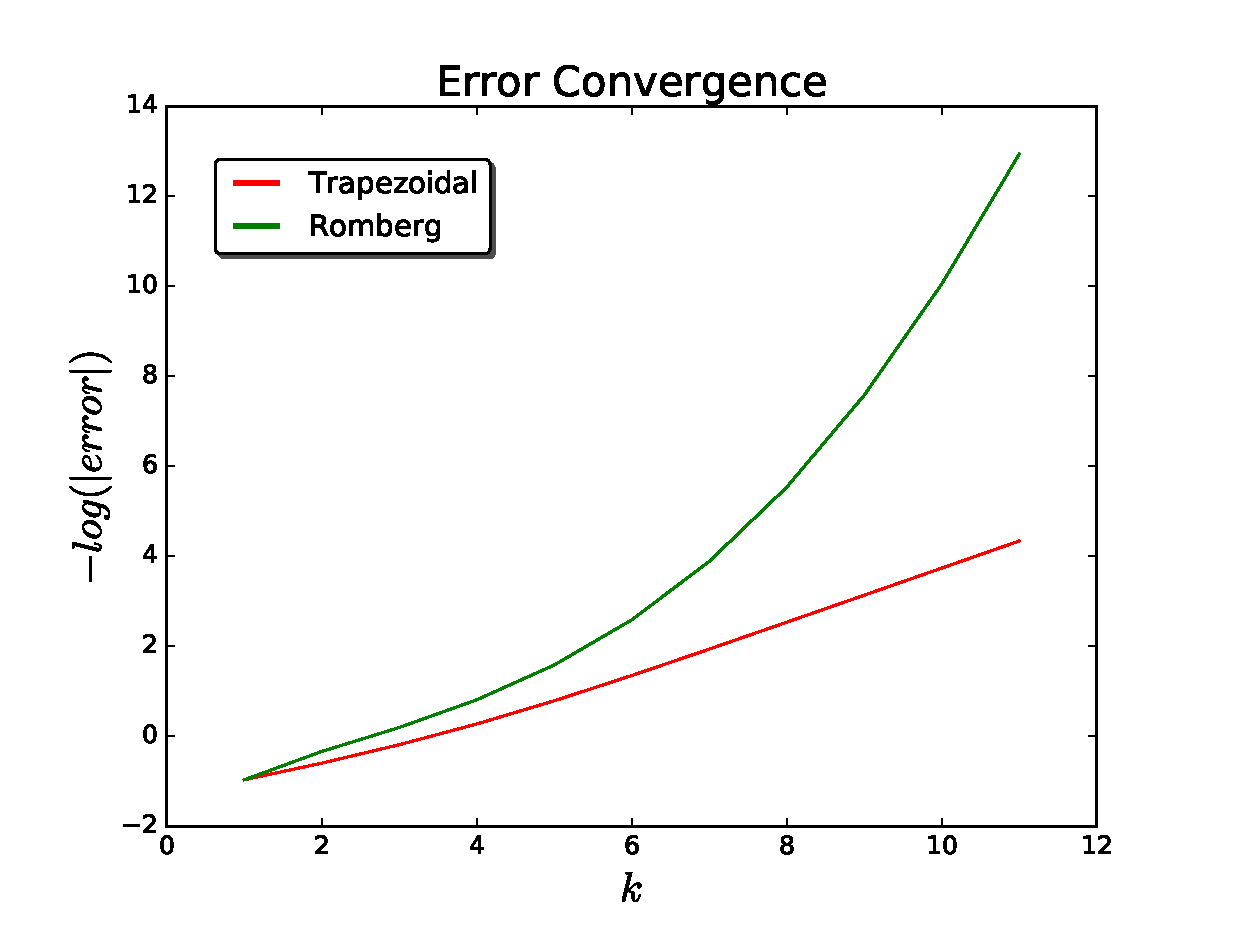
\includegraphics[width = 15cm]{convergence5.eps}
	\caption{Order of convergence for Trapezoidal with refinement and Romberg's method.}
\end{figure}

\newpage

\subsection{Function 6}
\vspace{1cm}
\begin{center}
	\begin{tabular}{|c|c|c|c|c|}
		\hline
		\texttt{Iteration} & \texttt{Refinement Result} & $error_{refinement}$ & \texttt{Romberg} $T_1^{iteration}$ & $error_{Romberg}$ \\ \hline \hline
		1 & -0.136099130644 & 0.049685405157 & -0.136099130644 & 0.049685405157 \\ \hline
		2 & -0.099140962160 & 0.012727236673 & -0.086821572665 & 0.000407847178 \\ \hline
		3 & -0.089618374887 & 0.003204649399 & -0.086419019560 & 0.000005294073 \\ \hline
		4 & -0.087216402199 & 0.000802676712 & -0.086413766931 & 0.000000041444 \\ \hline
		5 & -0.086614490884 & 0.000200765397 & -0.086413725635 & 0.000000000148 \\ \hline
		6 & -0.086463922876 & 0.000050197388 & -0.086413725488 & 0.000000000000 \\ \hline
		7 & -0.086426275212 & 0.000012549725 & -0.086413725487 & 0.000000000000 \\ \hline
		8 & -0.086416862942 & 0.000003137455 & -0.086413725487 & 0.000000000000 \\ \hline 
	\end{tabular}
	\vskip .25cm
	{Results and errors for Trapezoidal with refinements and the diagonal elements of Romberg's triangle.}
\end{center}

\begin{figure}[H]
	\centering
	\includegraphics[width = 15cm]{convergence6.eps}
	\caption{Order of convergence for Trapezoidal with refinement and Romberg's method.}
\end{figure}

\newpage

\section{Conclusion}

In this program we derived an analytical error form for the extrapolation methods $I_{new} = \frac{9}{5}I_{ss} - \frac{4}{5}I_{sf}$ and $I_{new} - \frac{7}{15}I_{sf} + \frac{8}{15}I_{o2}$ and showed that this method increases the order of infinitesimal, power of derivative, and degree of exactness. It was also shown that to be a Newton Cotes method it must interpolate at uniform mesh points. The former is not Newton Cotes but the latter is (both are interpolatory quadrature by theorem 1). We then when numerically investigated Trapezoidal method with refinement vs Romberg method with six integrals. It was shown that after some iteration Romberg method not only achieved higher order of accuracy, it did so with considerably lower computational cost. This leads to a very effecient way to achieve desired accuracy without low overhead. 

\end{document}
